% Professional text-free logo from a coding-theory perspective
% Standalone TikZ source for presentation/tikzs/logo-coding-theory.pdf
\documentclass[tikz, border=14pt]{standalone}

\usepackage{xcolor}

\usetikzlibrary{
  arrows.meta,
  calc,
  shapes.geometric
}

\definecolor{inkC}{HTML}{101A24}
\definecolor{paperC}{HTML}{F8FBFC}
\definecolor{gridC}{HTML}{DCEAEC}
\definecolor{codeC}{HTML}{008C8C}
\definecolor{codeDarkC}{HTML}{006A70}
\definecolor{fieldC}{HTML}{3155A4}
\definecolor{cryptoC}{HTML}{B87511}
\definecolor{errC}{HTML}{D33F49}

\begin{document}
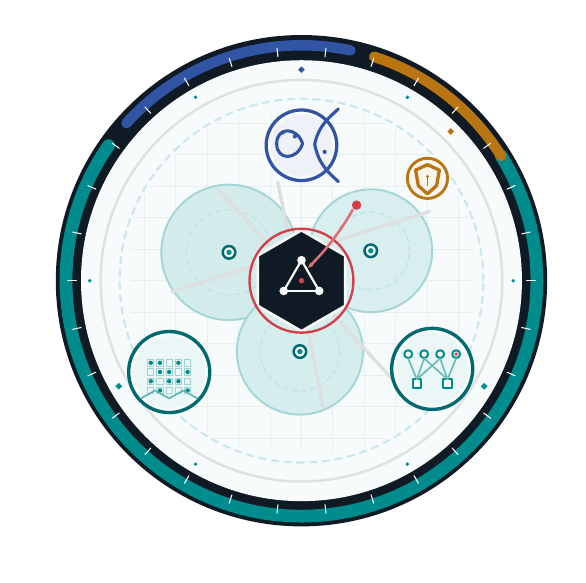
\begin{tikzpicture}[
  x=1cm,
  y=1cm,
  line cap=round,
  line join=round
]

\def\Rbadge{3.12}
\def\Rinner{2.80}
\coordinate (O) at (0,0);

% Outer badge: coding theory is the dominant layer.
\fill[inkC] (O) circle (\Rbadge);
\draw[codeC, line width=4.6pt] (145:2.99) arc[start angle=145, end angle=392, radius=2.99];
\draw[fieldC, line width=3.8pt] (78:2.99) arc[start angle=78, end angle=138, radius=2.99];
\draw[cryptoC, line width=3.8pt] (32:2.99) arc[start angle=32, end angle=72, radius=2.99];
\fill[paperC] (O) circle (\Rinner);
\draw[inkC!13, line width=0.9pt] (O) circle (2.55);
\draw[codeC!20, line width=0.8pt, dash pattern=on 2.5pt off 2.1pt] (O) circle (2.31);

% Rim ticks and check marks.
\foreach \ang in {0,12,...,348}{
  \draw[paperC!58, line width=0.38pt] (\ang:2.86) -- (\ang:2.97);
}
\foreach \ang in {0,60,...,300}{
  \fill[codeC] (\ang:2.69) circle (0.024);
}

% Faint coordinate space.
\begin{scope}
  \clip (O) circle (2.27);
  \foreach \x in {-2.0,-1.6,...,2.0}{
    \draw[gridC!72, line width=0.34pt] (\x,-2.16) -- (\x,2.16);
  }
  \foreach \y in {-2.0,-1.6,...,2.0}{
    \draw[gridC!72, line width=0.34pt] (-2.16,\y) -- (2.16,\y);
  }
\end{scope}

% Hamming balls around codewords.
\foreach \x/\y/\r/\opa in {-0.92/0.36/0.86/17, 0.88/0.38/0.78/15, -0.02/-0.90/0.80/16}{
  \fill[codeC!\opa] (\x,\y) circle (\r);
  \draw[codeC!36, line width=0.70pt] (\x,\y) circle (\r);
  \draw[codeC!25, line width=0.45pt, dash pattern=on 1.8pt off 1.6pt]
    (\x,\y) circle ({0.63*\r});
}

% Decision boundaries.
\draw[inkC!14, line width=1.25pt] (-0.30,1.25) -- (0.28,-1.62);
\draw[inkC!14, line width=1.25pt] (-1.65,-0.14) -- (1.63,0.88);
\draw[inkC!14, line width=1.25pt] (-1.05,1.15) -- (1.20,-1.30);

% Codeword centers.
\foreach \p in {(-0.92,0.36),(0.88,0.38),(-0.02,-0.90)}{
  \fill[paperC] \p circle (0.080);
  \draw[codeDarkC, line width=0.90pt] \p circle (0.080);
  \fill[codeC] \p circle (0.034);
}

% Central syndrome/decoder core.
\node[
  regular polygon,
  regular polygon sides=6,
  rotate=30,
  minimum size=1.28cm,
  inner sep=0pt,
  fill=inkC,
  draw=paperC,
  line width=0.95pt
] at (O) {};
\draw[errC, line width=0.85pt] (O) circle (0.66);

\coordinate (s1) at (90:0.26);
\coordinate (s2) at (210:0.26);
\coordinate (s3) at (330:0.26);
\foreach \a/\b in {s1/s2,s2/s3,s3/s1}{
  \draw[paperC!82, line width=0.78pt] (\a) -- (\b);
}
\foreach \p in {s1,s2,s3}{
  \fill[paperC] (\p) circle (0.055);
}
\fill[errC] (O) circle (0.035);

% Received word and nearest-neighbor correction.
\fill[errC] (0.70,0.96) circle (0.060);
\draw[errC!75, line width=0.92pt, -{Stealth[length=2.25pt]}]
  (0.65,0.90) .. controls (0.47,0.58) and (0.27,0.35) .. (0.08,0.16);

% Parity-check Tanner graph satellite.
\begin{scope}[shift={(1.66,-1.12)}, scale=0.78]
  \fill[paperC] (0,0) circle (0.66);
  \fill[codeC!8] (0,0) circle (0.58);
  \draw[codeDarkC, line width=1.22pt] (0,0) circle (0.66);
  \foreach \x in {-0.39,-0.13,0.13,0.39}{
    \fill[paperC] (\x,0.24) circle (0.064);
    \draw[codeC, line width=0.72pt] (\x,0.24) circle (0.064);
  }
  \foreach \x in {-0.25,0.25}{
    \fill[paperC] ({\x-0.070},-0.31) rectangle ({\x+0.070},-0.17);
    \draw[codeC, line width=0.72pt] ({\x-0.070},-0.31) rectangle ({\x+0.070},-0.17);
  }
  \foreach \a/\b in {-0.39/-0.25,-0.13/-0.25,-0.13/0.25,0.13/-0.25,0.13/0.25,0.39/0.25}{
    \draw[codeC!60, line width=0.58pt] (\a,0.17) -- (\b,-0.17);
  }
  \fill[errC] (0.39,0.24) circle (0.030);
\end{scope}

% Generator-matrix satellite without glyphs.
\begin{scope}[shift={(-1.68,-1.16)}, scale=0.78]
  \fill[paperC] (0,0) circle (0.66);
  \fill[codeC!8] (0,0) circle (0.58);
  \draw[codeDarkC, line width=1.22pt] (0,0) circle (0.66);
  \foreach \x in {-2,-1,0,1,2}{
    \foreach \y in {-2,-1,0,1}{
      \draw[codeC!38, line width=0.35pt]
        ({0.15*\x-0.052},{0.15*\y-0.052}) rectangle
        ({0.15*\x+0.052},{0.15*\y+0.052});
    }
  }
  \foreach \x/\y in {-2/1,-1/1,1/1,-1/0,0/0,2/0,-2/-1,0/-1,1/-1,-1/-2,2/-2}{
    \fill[codeC] ({0.15*\x},{0.15*\y}) circle (0.036);
  }
  \draw[codeC!64, line width=0.58pt] (-0.46,-0.43) -- (-0.23,-0.30)
    -- (0,-0.43) -- (0.23,-0.30) -- (0.46,-0.43);
\end{scope}

% Algebraic-code origin: small curve feeding the code space.
\begin{scope}[shift={(0,1.72)}, scale=0.70]
  \fill[paperC] (0,0) circle (0.64);
  \fill[fieldC!8] (0,0) circle (0.56);
  \draw[fieldC, line width=1.18pt] (0,0) circle (0.64);
  \draw[fieldC, line width=1.12pt]
    (-0.45,0.03)
      .. controls (-0.45,0.34) and (-0.08,0.34) .. (0.02,0.03)
      .. controls (-0.08,-0.28) and (-0.45,-0.28) .. (-0.45,0.03);
  \draw[fieldC, line width=1.12pt]
    (0.24,0.02) .. controls (0.31,0.36) and (0.52,0.52) .. (0.67,0.66);
  \draw[fieldC, line width=1.12pt]
    (0.24,0.02) .. controls (0.31,-0.36) and (0.52,-0.52) .. (0.67,-0.66);
  \foreach \p in {(-0.34,0.23),(-0.12,0.16),(0.42,-0.12)}{
    \fill[fieldC] \p circle (0.038);
  }
\end{scope}

% Cryptographic application: small shield.
\begin{scope}[shift={(1.60,1.30)}, scale=0.58]
  \fill[paperC] (0,0) circle (0.44);
  \fill[cryptoC!8] (0,0) circle (0.37);
  \draw[cryptoC, line width=1.05pt] (0,0) circle (0.44);
  \draw[cryptoC, line width=1.18pt]
    (0,0.30) -- (0.26,0.18) -- (0.20,-0.16) -- (0,-0.34)
    -- (-0.20,-0.16) -- (-0.26,0.18) -- cycle;
  \fill[cryptoC] (0,0.04) circle (0.035);
  \draw[cryptoC, line width=0.62pt] (0,0.00) -- (0,-0.15);
\end{scope}

% Rim separators.
\foreach \ang/\C in {90/fieldC, 210/codeC, 330/codeC, 45/cryptoC}{
  \node[
    regular polygon,
    regular polygon sides=4,
    rotate=45,
    fill=\C,
    minimum size=0.085cm,
    inner sep=0pt
  ] at (\ang:2.68) {};
}

\end{tikzpicture}
\end{document}
